\section{Cancer}
        Cancer is an illness caused by the uncontrolled division and spreading of normal cells~\cite{whatiscancer2021} unlike other diseases, cancer is caused by our own bodies and not by foreign entities, and it is one of the biggest causes of death among human beings nowadays (Table ~\ref{tab:cancerStat}) and that is because of the ineffectiveness of traditional treatment methods such as hormones, surgery, radiation, and chemotherapy~\cite{mahsa2022}. their ineffectiveness is due to there side effects that lead the body to deteriorate more and more. but it is worth mentioning that there are some new methods and approaches being developed by researchers, a couple of those methods are the study of stem cells in relation to cancer cells and the study of the normal cells that the cancer cells came from which are called "Cancer Origin Cells", the latter approach proposes that we should study these origin cells because of their big similarities with cancer cells which will give us a roadmap to its diagnosis and therapy~\cite{rachita2021} 
\begin{table}[htbp]
\begin{center}
\begin{tabular}{|c||c|}
Deaths in 2020 & nealry 10 million \\
\hline
\textbf{Type} & \textbf{New Cases} (millions) in 2020 \\
\hline
Breast &  2.26\\
\hline
Lung &  2.21\\
\hline
Colon and Rectum & 1.93 \\
\hline
Prostate & 1.41 \\
\hline
Skin &  1.20 \\
\hline
Stomach & 1.09 \\
\end{tabular}
\end{center}
\caption{Cancer Statistic ~\cite{cancerStat}}
\label{tab:cancerStat}
\end{table}
\subsection{Origin}
        One of the theories that discuss this is the "carcinogenesis multi-hit theory " which stipulates that for cancer to emerge there are some conditions (hits) that need to be satisfied these hits are produced by genetic mutations (figure ~\ref{fig:mutations}) or rearrangements (figure ~\ref{fig:reaarangement}) that occur over many years and the number of hits necessary is minimal ranging from 3 to 7 only~\cite{rachita2021}. but it is only fair to mention that there are some exceptions to the rule as there are some cancers caused by only one hit. and to go a step further these mutations can be caused by various elements in our environment such as chemicals in tobacco, ultraviolet rays...etc~\cite{whatiscancer2021}
%----------------------figure mutation-----------------------------
\begin{figure}[htbp]
\begin{center}
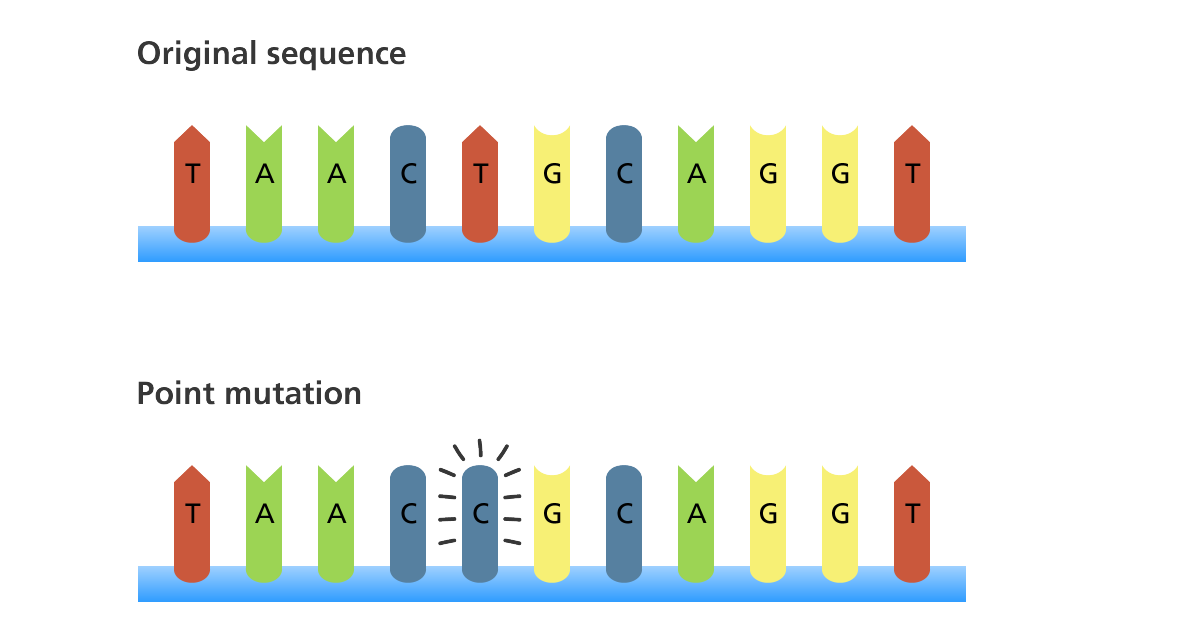
\includegraphics[width=15cm]{./chapter-01-general-medical-information/mutation.png}
\end{center}
\caption{DNA Mutation ~\cite{mutations}}
\label{fig:mutations}
\end{figure}
%----------------------figure rearrangements-----------------------------
\begin{figure}[htbp]
\begin{center}
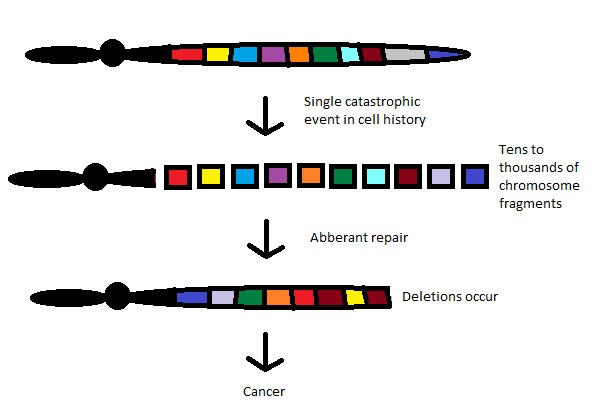
\includegraphics[width=15cm]{./chapter-01-general-medical-information/dna-rearrangement.png}
\end{center}
\caption{DNA Rearrangements ~\cite{reaarangement}}
\label{fig:reaarangement}
\end{figure}
\subsection{Types}
        \subsubsection{according to fatality}
        \begin{description}
            \item[benign tumors]
            are not very harmful because they do not spread to other organs and do not invade nearby tissue, and after removal, they usually don't grow back~\cite{whatiscancer2021} as shown in figure ~\ref{fig:benignMalignant}
            \item[malignant tumors]
            fatal if not treated, because they travel to distant places and form other tumors and invade nearby tissue~\cite{whatiscancer2021} which makes it very hard to remove all its parts, as shown in figure ~\ref{fig:benignMalignant}
%-----------benign malignant------------------------
\begin{figure}[htbp]
\begin{center}
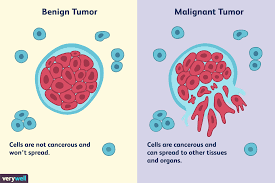
\includegraphics[width=15cm]{./chapter-01-general-medical-information/benign-malignant.png}
\end{center}
\caption{Benign and Malignant tumors  ~\cite{benignMalignant}}
\label{fig:benignMalignant}
\end{figure}
        \end{description}
            \subsubsection{according to origin}
            cancer is also categorized according to where it originated or its origin cells, in this category, there are over 100 types because of the different places it can appear (lung cancer, brain cancer ...)and the different origin cells that it can come from~\cite{whatiscancer2021}.
            \begin{description}
                \item[carcinoma]
                most common type formed by epithelial cells 
                \item[sarcoma]
                form in bone and soft tissue
                \item[leukemia]
                form in bone marrow, this type does form a tumor but travels in the blood 
                \item[melanoma]
                formed by melanocytes (cells that make melanin that gives the skin its color)
                ...etc
            \end{description}
